\documentclass[runningheads]{llncs}
%\documentclass{article}

\usepackage{textcomp}
\usepackage{framed}
\usepackage{amsmath}
\let\proof\relax
\let\endproof\relax
\usepackage{amsthm}
\usepackage{mathtools}
\usepackage{hyperref}
\usepackage{fnpct}

\makeatletter

\DeclareRobustCommand*{\lyxarrow}{%
\@ifstar
{\leavevmode\,$\triangleleft$\,\allowbreak}
{\leavevmode\,$\triangleright$\,\allowbreak}}

\makeatother

\begin{document}

\title{A Tutorial on Verifying \texttt{LinkedList} using KeY}
\author{{Hans-Dieter} A. Hiep\orcidID{0000-0001-9677-6644}\footnote{Corresponding author: \texttt{hdh@cwi.nl}}\and Jinting Bian\and\\
Frank S. de Boer\and Stijn de Gouw}
\authorrunning{H.A. Hiep, J. Bian, et al.}
\institute{CWI, Science Park 123, 1098 XG Amsterdam, The Netherlands\\
\email{\{hdh,j.bian,frb,stijn.de.gouw\}@cwi.nl}}

\maketitle

\begin{abstract}
This is a tutorial paper on using KeY to demonstrate formal verification of state-of-the-art, real software. We explain in sufficient detail for a beginning user of JML and KeY, the specification and verification of part of a corrected version of the \texttt{java.util.LinkedList} class of the Java Collection framework.
\end{abstract}

\keywords{KeY, Java Modeling Language, cyclic data structure, case study}

\section{Introduction}

Software libraries are the building blocks of many programs that run on the devices of many more users every day. The functioning of a system may rely for a large part on its used software libraries. A small error present in a heavily-used software library could lead to serious unwanted outcomes, such as system outages and failures. Using root cause analysis, one could find from a system failure the errors that have caused it. But root cause analysis can only applied \emph{after} a failure has happened. To prevent failures from happening in the first place, correctness is of the utmost importance. Although establishing program correctness seems to be an expensive activity, it may be worthwhile for critical software libraries, such the standard library that all programs rely on.

This tutorial intends to show how we take an existing Java program that is part of the Java standard library, and study it closely to increase our understanding of it. If we are only interested in showing the presence of an issue with the program, e.g.~that it lacks certain functionality, it suffices to show an example run which behaves unexpectedly. But to reach the conclusion that no unexpected behavior ever results from running the program, first requires a precise specification of what behavior one expects, and further requires a convincing argument that all possible executions of the program exhibit that behavior.

We take a formal approach to both specification and reasoning about programs, allowing us to increase the reliability of our reached conclusions. In particular, the specifications we write are expressed in the Java Modeling Language (JML), and our reasoning is tool-supported and partially automated by KeY. To the best of the authors' knowledge, KeY is the only tool that supports enough features of the Java programming language for reasoning about realistic programs, of which its run-time behavior crucially depends on the presence of such features, such as: dynamic object creation, exception handling, integer arithmetic with overflow, \texttt{for} and \texttt{foreach} loops with early returns, nested classes (both static and non-static), inheritance, polymorphism, erased generics, etc.

As a demonstration of applying KeY to real software, we will focus on Java's \texttt{LinkedList} class for two reasons. First, a (doubly-)linked list is a well-known basic data structure for storing and maintaining unbounded data, and has many applications: for example, in Java's secure sockets implementation. Second, it has turned out that there is a 20-year-old bug lurking in its program, that might cause security issues on large memory systems, caused by the overflow of a field that caches the length of the list. Our specification and verification effort will be aimed at establishing the absence of this bug from a repaired program.

In this tutorial, we see how to set-up a project and configure the KeY tool, and outline the general workflow that we follow (Section~\ref{sec:setup}). We study the source code of the \texttt{LinkedList}, and get an intuitive grasp of its essential structure: how the various instances of this class look like, and how some essential methods operate on these instances (Section~\ref{sec:linkedlist}).

To keep this presentation reasonably short, we focus only on the methods \texttt{add} and \texttt{remove}. We shall formulate, based on previous intuition, a \emph{class invariant} in JML that expresses a property that is true of every instance and must remain true after executing our methods (Section~\ref{sec:class-invariant}). We use the invariant in formulating a \emph{method contract} for the \texttt{add} method that describes its expected behavior and we verify that its implementation is correct (Section~\ref{sec:add}).

The difficulty level increases after we specify the \texttt{remove} method (Section~\ref{sec:remove}), as its verification requires more work than before. Certain lemmas are needed: one that follows from the invariant (Section~\ref{sec:acyclicity}), one that implies the invariant (Section~\ref{sec:unlinking}), and \emph{loop invariants} (Section~\ref{sec:loop-invariant}).

Some other methods of \texttt{LinkedList} are left as exercises to the reader: finding their specifications and proving them correct is not trivial, but are done in a similar way. We conclude with remaining methods that still pose challenges.

\section{Set-up}\label{sec:setup}
\subsection{Project files}
\subsection{KeY settings}

To produce proofs in KeY, the first step is to set-up KeY's taclet base to make use of particular groups of rules that correctly model Java's integer overflow semantics. This has to be done only once, as these taclet settings are stored per computer user. Sometimes, KeY overwrites or corrupts these settings if different versions are used: in that case, one can remove ??? from the user's home directory.

Start up KeY and load an example (File\lyxarrow Load Example\lyxarrow choose the first example). Then open Options\lyxarrow Taclet Options, and configure them as follows:

\begin{description}
\item [JavaCard] Off
\item [Strings] On
\item [Assertions] Safe
\item [BigInt] On
\item [Initialization] Disable static initialization
\item [Integer Rules] Java semantics
\item [Integer Simplification Rules] Full
\item [Join Generate Is Weakening Goal] Off
\item [Model Fields] Treat as axiom
\item [More Sequence Rules] On
\item [Permissions] Off
\item [Program Rules] Java
\item [Reach] On
\item [Runtime Exceptions] Ban
\item [Sequences] On
\item [Well-definedness Checks] Off
\item [Well-definedness Operator] L
\end{description}

After setting these taclet options, they become effective after loading the next problem. We do that now: the main proof file \texttt{LinkedList.key} can be loaded, and a contract selection window opens up, showing a class hierarchy and its methods. Selecting a method shows its method contracts. There may be no method contracts when no specification have been written. After following the examples below, method contracts can be selected in this window.

\subsection{Workflow}


\section{\texttt{java.util.LinkedList}}\label{sec:linkedlist}

This class has three attributes: a \texttt{size} field, which stores the number of elements in the list, and two
fields that store a reference to the \texttt{first} and \texttt{last} node. Internally, it uses the private static nested \texttt{Node} class to represent the items in the list. A static nested private class behaves like a top-level class, except that it is not visible outside the enclosing class (\texttt{LinkedList}, in this case). Nodes are doubly linked; each node is connected to the preceding (field \texttt{prev}) and succeeding node (field \texttt{next}). These fields contain \texttt{null} in case no preceding or succeeding node exists. The data itself is contained in the \texttt{item} field of a node.

Source
Constructor, add method, remove method

\subsection{Expected behavior}
Pictures of instances

Pictures of adding

Pictures of removing

\subsection{Bugfix}
Short description of bug

Short fix to problem (checkSize)

\section{Class invariant}\label{sec:class-invariant}

Each linked list consists of a sequence of nodes. Sequences are finite, indexing of sequences starts at zero, and we write $\sigma[i]$ to mean the $i$th element of some sequence $\sigma$. A \emph{chain} is a sequence $\sigma$ of nodes of length $n>0$ such that: the \texttt{prev} reference of the first node $\sigma[0]$ is \texttt{null}, the \texttt{next} reference of the last node $\sigma[n-1]$ is \texttt{null}, the \texttt{prev} reference of node $\sigma[i]$ is node $\sigma[i-1]$ for every index $0<i<n$, and the \texttt{next} reference of node $\sigma[i]$ is node $\sigma[i+1]$ for every index $0\leq i < n-1$. The \texttt{first} and \texttt{last} references of a linked list are either both \texttt{null} to represent the \emph{empty} linked list, or there is some chain $\sigma$ between the \texttt{first} and \texttt{last} node, viz.~$\sigma[0]=\mathtt{first}$ and $\sigma[n-1]=\mathtt{last}$. Figure \ref{fig:linkedlist} shows example instances.
Also see standard literature such as Knuth's \cite[Section 2.2.5]{knuth1997art}.

\begin{figure}[t]
  \centering
  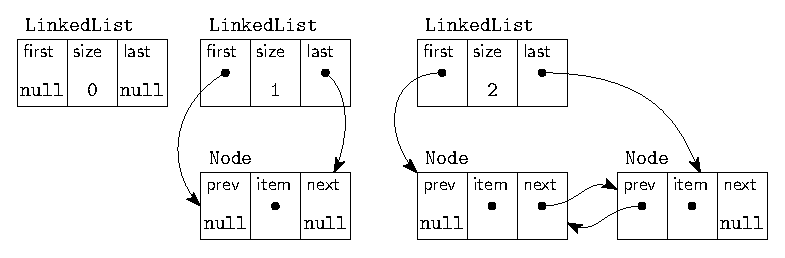
\includegraphics[scale=0.75]{figures/linkedlist1.eps}
  \caption{Three example linked lists: empty, with a chain of one node, and with a chain of two nodes. Items themselves are not shown.}
  \label{fig:linkedlist}
\end{figure}

\subsection{Cached vs. real size}
\subsection{Ghost node list}
\subsection{Reference structure}
\section{The \texttt{add} method}\label{sec:add}
\section{The \texttt{remove} method}\label{sec:remove}
\section{Acyclicity}\label{sec:acyclicity}
\section{Unlinking}\label{sec:unlinking}
\section{Loop invariants}\label{sec:loop-invariant}
\section{Conclusion}

\bibliographystyle{splncs04}
\bibliography{base}

\end{document}
\endinput
